% Design
% Requires in preamble: \usepackage{tikz}  \usetikzlibrary{arrows.meta,positioning}
\begin{figure*}[t]
  \centering
  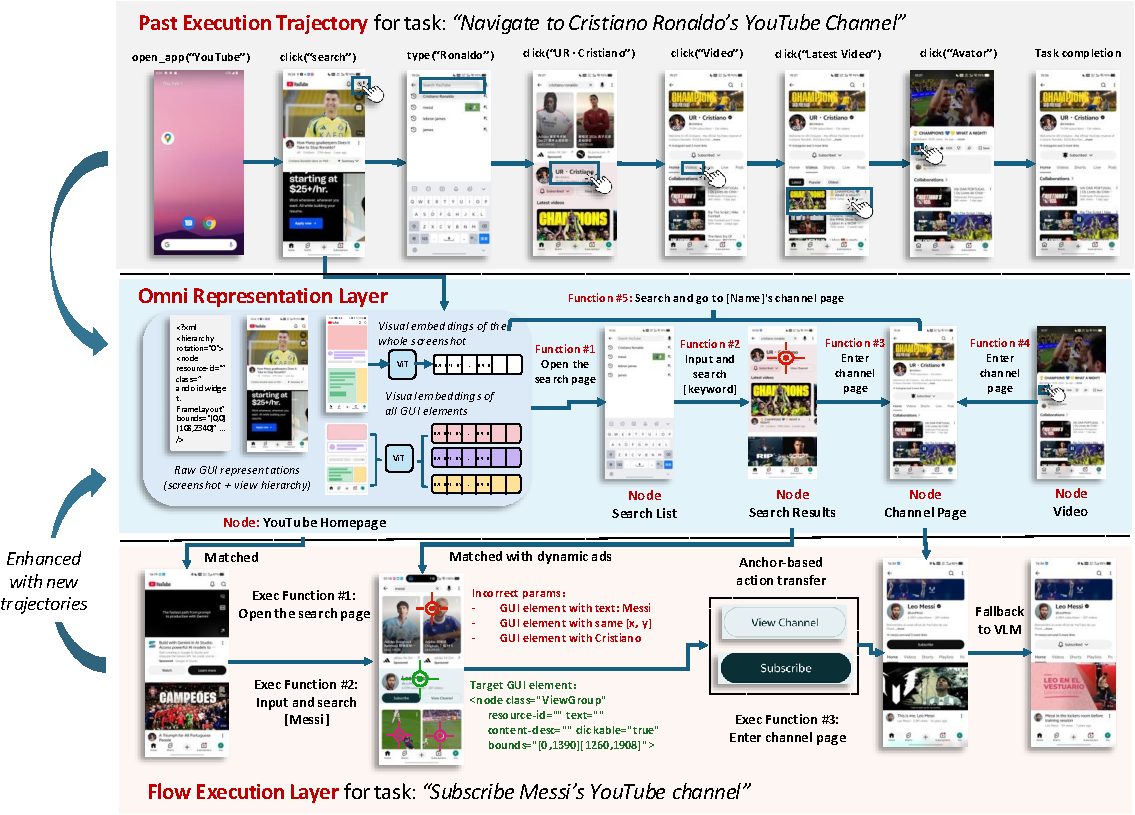
\includegraphics[width=0.94\textwidth]{figs/demo.pdf}
  \vspace{-0.5em}
  \caption{Demonstration of how a task execution trajectory is transformed into memory and how that memory is adaptively utilized in online execution environments.}
  \label{fig:demo}
  \vspace{-0.6em}
\end{figure*}

\begin{figure*}[t]
  \centering
  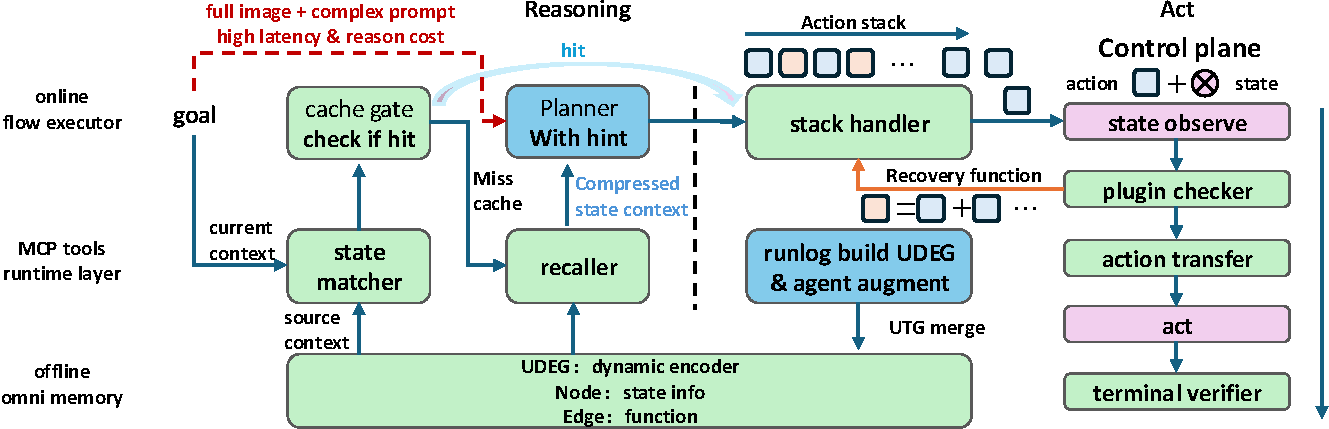
\includegraphics[width=0.94\textwidth]{figs/F20_system_design.pdf}
  \vspace{-0.5em}
  \caption{\wzw{}{System design overview.
  OmniFlow builds a Function Store whose assets are API-like Functions synthesized from successful GUI executions.
  The store induces a sparse UDEG: privacy-safe GUI-state nodes index where Functions can be invoked, and Function edges record executable task effects.
  \textsc{Omni} recalls a compatible Function through this state index; \textsc{Flow} executes it through a single observe-check-transfer-act stack and writes accepted run logs back into the Function Store.}}
  \label{fig:pptx-system-design-overview}
  \vspace{-0.6em}
\end{figure*}

\section{System Design}
\label{sec:design}

\subsection{Architecture and Workflow}
\label{sec:design-overview}

\sysname consists of two layers.
(1) \textsc{Omni} representation layer manages history traces and converts them into reusable and callable memory functions.
(2) \textsc{Flow} execution layer  executes recalled Functions and VLM-generated actions on the live device. 



% ───────────────────────────────────────────────────────────────────────────
\subsection{\textsc{Omni} Representation Layer}
\label{sec:design-offline}



\textsc{Omni} exposes two interfaces: \emph{recall} retrieves executable Functions from the Function Store, and \emph{Update} ingests execution logs into the Function Store for offline enhancement.

\textbf{UDEG.} \sysname builds a UDEG (Universal-Device-Execution Graph) to support cross-device and cross-user Function reuse. UDEG nodes are clusters of GUI states, and edges are executable Functions.

Some works use UTG (UI transition graph) to represent the app state space, but mobile GUI states are often highly dynamic and user-specific, which makes UTG need to be updated frequently. Instead of storing raw screenshots or raw XML, UDEG nodes store compact feature vectors that capture the visual, structural, geometric, and interaction cues of the GUI state. \sysname uses xml-feature compactor to acomplish page embedding because vision-embedding-model is expensive and privacy-sensitive, while xml features are cheap and structured. We prove in \S\ref{sec:evaluation} that this representation is sufficient for high-accuracy page matching and Function recall.

For each element, it builds a 64-dimensional feature vector from two sources:
screenshot-derived visual cues, such as icons, labels, and clickable regions, and view-hierarchy-derived cues, such as widget class, interaction flags, bounds, and tree position.

The element vectors are pooled into a compact page vector for approximate lookup.
For each UI element $e_i$, \sysname builds an element vector
\[
  \mathbf{v}_i=\phi(e_i),
\]
where $\phi(\cdot)$ combines visible cues and accessibility-structure cues:
content hash, element type, interaction flags, subtree shape, hierarchy,
resource-id hints, and normalized geometry.
\sysname then groups elements into UI subspaces, each defined by a
predicate over the element and its page context:
\[
  \mathcal{S}_k(X)=\{e_i \in X \mid c_k(e_i,X)=1\}.
\]
For each subspace, \sysname computes a weighted vector:
\[
  \mathbf{p}_k(X)=
  \frac{\sum_{e_i\in \mathcal{S}_k(X)} \alpha_{ik}\mathbf{v}_i}
       {\sum_{e_i\in \mathcal{S}_k(X)} \alpha_{ik}}.
\]
The page vector is the weighted concatenation of these subspace vectors:
\[
  \mathbf{p}(X)=
  \frac{[w_1\mathbf{p}_1;\ldots;w_K\mathbf{p}_K]}{W_P},
  \qquad
  W_P=\sum_{k=1}^{K}w_k .
\]

% 这种方法的优势：top-1 accuracy很高，可以快速定位到已有的page，从而实现：1、召回可能触发的Function；2、高效获取相似历史页面上的操作对，来增强当前的操作.
This method can quickly locate a matching page in the UDEG, which enables two key capabilities: (1) recalling Functions that can be invoked in the current GUI state, and (2) efficiently retrieving similar historical actions from the matched page to enhance the current operation. In \S\ref{sec:evaluation}, we demonstrate that this approach achieves high top-1 accuracy in page matching.

\textbf{Recall.} \sysname uses the current GUI state and task context to recall candidate Functions from the Function Store. When an observe cycle completes, \textsc{Omni} queries the UDEG index to retrieve a set of potentially invokable Functions. These Functions are then passed to a lightweight cache gate model that assesses their executability and fills in any required parameters. This approach leverages general knowledge for semantic similarity assessment and parameter completion, allowing the small model to perform effectively. Typically, a single invocation requires only a few milliseconds, enabling rapid decision-making in real-time execution scenarios.

\textbf{Update.} Updater ingests execution logs into the Function Store to enhance the executability and generalization of Functions. Upon receiving a raw execution trace, it is first processed by an enhancement module that performs offline augmentation. Through backend agent calls, key actions are identified, semantic information of the actions is extracted, and structured documentation is generated for subsequent model deployment. This process ensures that the Function Store remains up-to-date with the latest execution patterns and can effectively support future task executions.


% ───────────────────────────────────────────────────────────────────────────
\subsection{\textsc{Flow} Execution Layer}
\label{sec:design-online}

\textsc{Flow} is the execution layer that grounds recalled Functions and VLM-generated actions on the live device. It provides a action stack for pending actions, and execute each action through a observe-checker-transfer-act loop. 

% 当动作到来时，我们用了两个组件增强其执行性能。我们首先利用checker将agent对过去执行历史的观察沉淀成可执行规则，在新的环境下校验，其次利用transfer将已有的动作的重定位.
When an action arrives, we enhance its execution performance using two components. First, we utilize checkers to distill the agent's observations of past execution history into executable rules, which are then validated in the new environment. Second, we employ transfer to relocate existing actions to the current context.

% 在实际执行时，动作序列并不是固定的，而是会不断注入胶水动作，例如：关闭广告弹窗、关闭键盘弹出等。之前的工作常常需要fallback或者人工干预，但局部的错误段可以通过统一的规则管理。为了让一个function能够实现局部恢复，我们实现了checker，其核心思想是设计一套通用的工具集合，让执行器可以将自然语言和提示转换为固定动作。通过这一中间件，\sysname可以在历史离线增强的时候为function和node不断创建新的checker，捕捉错误信号，并在实际执行时复用.

\textbf{Plugin checkers.} During execution, the action sequence is not fixed and may be interleaved with interrupt actions, such as closing pop-ups or dismissing keyboards. Previous works often require fallback or manual intervention for such cases, but local errors can be managed through a unified set of rules. To enable local recovery for a Function, we implement checkers that serve as a middleware, converting natural language and prompts into fixed actions. This allows \sysname to continuously create new checkers for Functions and nodes during offline enhancement, capturing error signals and reusing them during actual execution.

On execution, each checker defines a configurable trigger over the current GUI state, the pending action, or the current execution context. 
When the trigger condition is met, the checker can either inject a corrective action into the pending action stack or abort the current Function execution. This mechanism allows for dynamic adaptation to unexpected GUI changes, ensuring that the execution remains robust and reliable even in the presence of environmental variability.

\textbf{Action transfer.} Traditional coordinate replay and selector replay rely on a single unstable consumption: the recorded point or the target element's own attributes. This is fragile on mobile GUIs, where elements often lack stable \texttt{resource-id}, visible text, or accessibility names, and where layouts shift across executions.


\sysname instead treats transfer as relation-aware matching between the
source and current context. Transfer maps a recorded source action in a recalled \texttt{Function} to an executable action on the live GUI state:

\[
\texttt{transfer}:(S,e,T)\mapsto e',
\]

where $S$ is the recorded source page, $e$ is the source action target, $T$ is the current page, and $e'$ is the target element to execute on the live device.
The design follows a common property of mobile GUI tasks.

It scores source and current elements with
element vectors, selects high-confidence one-to-one matches as
anchors, and lets each anchor vote for a compatible current target by projecting
the recorded action through the action--anchor relation.  Each vote combines
action similarity, anchor similarity, and action--anchor distance consistency
from bounds and parent links.  This makes transfer depend on stable local and
global UI structure, such as cards, search bars, tab bars, section headers, and
navigation controls, while avoiding an early commitment to global anchors that
do not explain the current action.






\begin{algorithm}[t]
\caption{Anchor-based action transfer for one recorded action}
\label{alg:anchor-transfer}
\small
\begin{algorithmic}[1]
\Require source page $S$; current page $T$; recorded source action element $e$
\Ensure executable target action or \textsc{Abstain}
\State $M \gets$ pairwise element-similarity matrix between $S$ and $T$
\State $A \gets$ high-similarity one-to-one pairs $(a,a')$ from $M$
\State $V \gets$ empty vote table over elements in $T$
\ForAll{$(a,a') \in A$}
  \State $\hat{x} \gets$ project $e$ through the path $e \rightarrow a \rightarrow a'$
  \State $C \gets$ compatible current elements near $\hat{x}$
  \ForAll{$e' \in C$}
    \State $r \gets$ relation consistency between $(e,a)$ and $(e',a')$
    \State $v \gets \textsc{Sim}(e,e') \cdot \textsc{Sim}(a,a') \cdot r$
    \State $V[e'] \gets V[e'] + v$
  \EndFor
\EndFor
\State $c^* \gets$ highest-vote element in $V$
\If{$c^*$ has enough vote support and margin}
  \State \Return recorded action rebound to target element $c^*$
\Else
  \State \Return \textsc{Abstain}
\EndIf
\end{algorithmic}
\end{algorithm}